\documentclass[12pt,a4paper]{article}
\title{%
	Øving 1 \\
	\large IELET2003 - Elektroteknikk 2 \\
	}
\author{Gunnar Myhre, BIELEKTRO}

\usepackage[utf8]{inputenc}
\usepackage[norsk]{babel}
\usepackage{pgfplots}
\usepackage[siunitx]{circuitikz}

\usepackage{graphicx}
\graphicspath{ {./images} }

\setlength\parindent{0pt}

\begin{document}
	\maketitle

  \section*{Oppgåve 1}
    \subsection*{a)}
      \begin{equation}
        U_{xy} = U_x - U_y = -5[V] - 8[V] = -13[V]
      \end{equation}
      Svaralternativ: \textbf{C}

    \subsection*{b)}
      For effekten i ein motstand gjeld forholdet
      \begin{equation}
        P = ui \rightarrow P = Ri^2 \rightarrow P = \frac{u^2}{R}
      \end{equation}
      effekten er proporsjonal med kvadratet av spenninga, med motstandens konduktans
      som korrelasjonskoeffisient.
      Svaralternativ: \textbf{B}

    \subsection*{c)}
      Om me kortslutter terminalane vert spenningsfallet over $R_2=0[V]$
      \begin{equation}
        i=\frac{u}{R} = \frac{50[V]}{10[\si{\kilo\ohm}]} = 5[\si{\milli\ampere]}
      \end{equation}
      Svaralternativ: \textbf{C}

    \subsection*{d)}
      Kjeldetransformerer og slår saman straumkjeldene
      \begin{center}
        \begin{circuitikz}[american] \draw
          (0,0) to[I, i=$i$] (0,2) -- (2,2)
                to[R, l=$3\si{\ohm}$, v=u] (2,0) -- (0,0)
          ;
        \end{circuitikz}
      \end{center}
      \begin{equation}
        u = Ri = 3[\si{\ohm}] \cdot \left(2 + \frac{8}{3}\right)[\si{\ampere}] = 14 [V]
      \end{equation}
      Svaralternativ: \textbf{B}

    \subsection*{e)}
      Proporsjonane må vere like for at spenningsdelinga skal vere lik, altså må $R=3\cdot10
      \si{\ohm} = 30\si{\ohm}$. Me kan også finne motstandsverdien vha. spenningsdeling
      \begin{equation}
        \frac{R_{20}}{R_{20} + R_{60}} = \frac{R_{10}}{R_{10} + R} \rightarrow
        R = R_{10}\frac{R_{20} + R_{60}}{R_{20}} - R_{10} = 30\si{\ohm}
      \end{equation}
      Svaralternativ: \textbf{B}

  \section*{Oppgåve 2}
    Finner $R_{th} = \frac{R_1R_2}{R_1 + R_2}$ ved å nulle ut kjelda. Finner $E_{th} =
    \frac{R_2}{R_1 + R_2}E$ vha. spenningsdeling.
    \begin{itemize}
      \item $R_{th} = 8,18 [\si{\kilo\ohm}]$
      \item $E_{th} = 5,45 [V]$
    \end{itemize}

  \section*{Oppgåve 3}
    Oppgåva lar seg lettare løyse vha. kjeldetransformasjon. Me får straumkjelder i
    parallell $2[A] + 8[A] = 10[A]$ og motstandar i parallell $\frac{12\cdot24}{12+24}
    [\si{\ohm}] = 8[\si{\ohm}]$. Kjeldetransponerer tilbake til spenningskjelde
    \begin{center}
      \begin{circuitikz}[american] \draw
        (0,0) to[V, l=$80V$, invert] (0,2)
              to[R, l=$8\si{\ohm}$] (4,2)
              to[R, l=$56\si{\ohm}$, v=u] (4,0) -- (0,0)
        ;
      \end{circuitikz}
    \end{center}
    \begin{equation}
      i = \frac{u}{r} = \frac{80[V]}{(8 + 56)[\si{\ohm}]} = 1,25[A]
    \end{equation}

  \section*{Oppgåve 4}
    Ved temperatur $T > \ang{0} K$ vil dei negativt lada elektrona og dei
    positivt lada hola diffundere i alle retningar. Tendensen over tid er at
    det P-dopa området (anode) vert \textit{positivt} ladd og det N-dopa
    området (katode) vert \textit{negativt} ladd, denne prosessen kallast
    \textit{rekombinasjon med majoritetsberarar}. I grenseområdet mellom anoden
    og katoden vil det vere eit underskot av majoritetsberarar
    (\textit{utarmingsområde}), som forårsaker eit elektrisk felt frå katoden
    mot anoden og fungerer som ein isolator. 
    \begin{itemize}
      \item Spenningssetting i leieretning (\textit{forward bias}): Utarmingsområdet
        skrumper inn, og gradvis vil isoleringstilstanden avta.
      \item Spenningssetting i sperreretning (\textit{reverse bias}): Utarmingområdet
        veks.
    \end{itemize}

    Denne asymetrien er vesentleg for halvledarkomponenter slik som diodar og transistorar.
    \begin{center}
      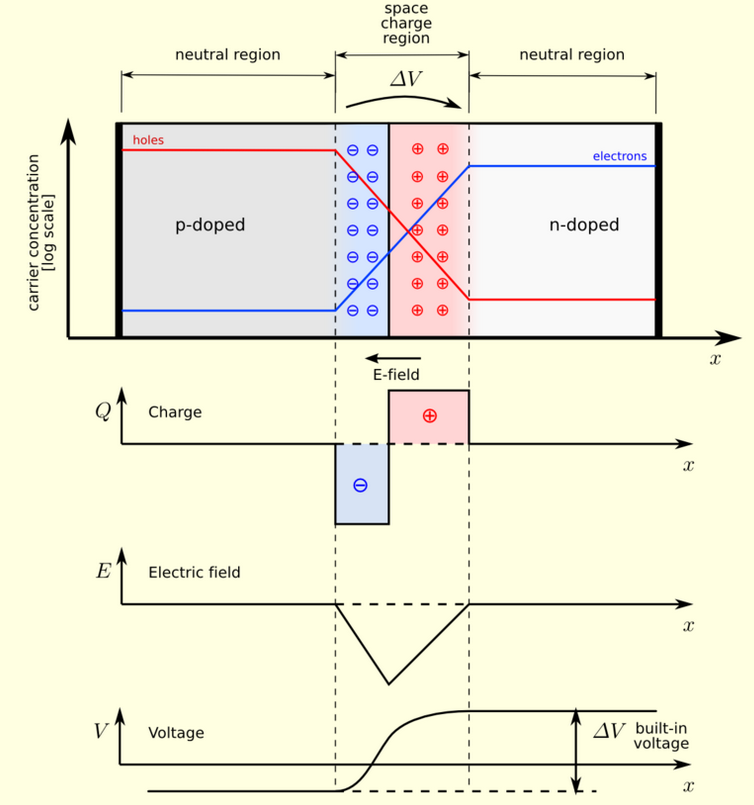
\includegraphics[scale=0.4]{01_04.png}
    \end{center}



\end{document}
